\chapter{Convergent-Beam Electron Diffraction} \label{chap:appendix-CBED}
If the specimen is illuminated by a parallel plane electron wave, electron diffraction, which is caused by electron scattering due to interaction with the atoms, occurs and the intensity in the far-field is given by:
\begin{equation}
  I\left(\vb{k}\right) = \lvert\mathcal{F}\left\{\psi_{\mathit{obj}}\left(\vb{k}\right)\right\}\rvert^2 \quad ; \quad \vb{k} = \frac{\theta}{\lambda},
\end{equation}
where $\psi_{\mathit{obj}}$ is the object wave modulated by the specimen, $\vb{k}$ the scattering vector in the detector plane and $\theta$ the scattering angle \cite{Hawkes2019,Williams2009}.

By choosing the (diffraction-limited) probe such that it is significantly larger than the electron source at the specimen, the probe described by the convergent electron beam can be considered as coherent \cite{Hawkes2019,Williams2009}. If the investigated specimen is crystalline, it therefore diffracts the electrons into discrete Bragg beams, which are broadened into discs when using the electron microscope in STEM~mode \cite{Hawkes2019,Williams2009}.
\newpage
Consequently, convergent-beam electron diffraction (CBED) allows for the measurement of the crystalline part of a specimen's thickness $t_{\mathit{CBED}}$ through a comparison with corresponding simulations (\cref{fig:CBED-comparison-simulation-thickness}).\footnote{All measurement data, simulations, analyses and plots were graciously provided by Dr.~Ines Häuser from the Humboldt University of Berlin.}
\begin{figure}[H]
  \centering
  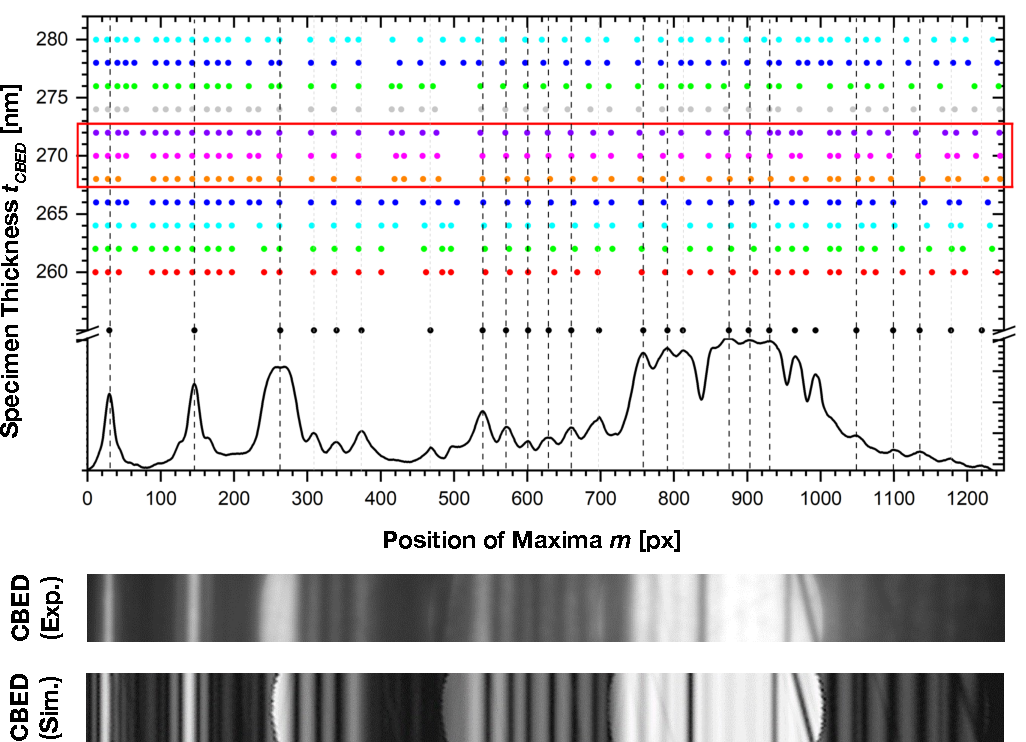
\includegraphics[width=\textwidth]{Figures/Specimen/pn-Junction/CBED-comparion-simulation-thickness.pdf}
  \caption{Determination of the specimen thickness $t_{\mathit{CBED}}$ from the comparison between CBED simulations and the experimental measurement. The thickness can be obtained by finding the corresponding simulation where the positions of the maxima $m$ of the HOLZ lines are in best agreement with the experimentally obtained diffraction pattern (indicated by the red rectangle).}
  \label{fig:CBED-comparison-simulation-thickness}
\end{figure}
For this purpose, the specimen is simulated with different thicknesses using the \emph{JEMS} software package \cite{JEMS}. By matching the position of the maxima $m$ of the higher-order Laue zones (HOLZ) lines, the crystalline part of the specimen thickness is determined to be $t_{\mathit{CBED}} = \SI{270 \pm 2}{\nm}$ (\cref{fig:CBED-comparison-simulation-thickness}, indicated by the red rectangle).
